\documentclass{VUMIFPSbakalaurinis}
\usepackage{algorithmicx}
\usepackage{algorithm}
\usepackage{algpseudocode}
\usepackage{amsfonts}
\usepackage{amsmath}
\usepackage{bm}
\usepackage{caption}
\usepackage{color}
\usepackage{float}
\usepackage{graphicx}
\usepackage{listings}
\usepackage{subfig}
\usepackage{wrapfig}
\usepackage{multirow}

% Titulinio aprašas
\university{Vilniaus universitetas}
\faculty{Matematikos ir informatikos fakultetas}
\department{Programų sistemų bakalauro studijų programa}
\papertype{Kursinis darbas}

\title{Šilumos laidumo uždavinio lygiagretinimas MIF klasteryje}
\titleineng{Parallelization of the steady-state heat problem on the MIF computing cluster}
\author{Mantas Petrikas}
\supervisor{dr. Rokas Astrauskas}
\date{Vilnius – \the\year}

% Nustatymai
% \setmainfont{Palemonas}   % Pakeisti teksto šriftą į Palemonas (turi būti įdiegtas sistemoje)
\bibliography{bibliografija}

\begin{document}
\maketitle



\tableofcontents


\sectionnonum{Įvadas}

Kompiuterinės simuliacijos yra svarbi modernių tyrimų dalis. 
Norint elektyviai atlikti sudėtingas simuliacijas, dažnai neužtenka vieno kompiuterio branduolio resursų, ir reikia paskirstyti darbą kelioms procesoriaus gijoms.
Tai galima padaryti išnaudojant centriniam procesoriuje esančius branduolius ir gijas, naudojant grafinius procesorių, ar pasitekiant superkompiuteriuose esančias sujungtus mazgus, taip išnaudojant daugiau nei vieną  centrinį ar grafinį procesorių.

Viena tipinė lygiagretino užduotis yra šilumos lygties sprendimas. 
Šilumos lygtis yra vienas iš Puasono lygties (ang. Poisson's equation) pritaikymo galimybių. 
Šios dalinės diferencialinės lygtys plačiai naudojamos fizikoje, sprendžiant elektrostatikos \cite{house2008analytic}, gravitacijos, magnetizmo \cite{blakely1996potential}, pastovios būsenos temperatūrų \cite {berntsson2001numerical} ir hidrodinamikos \cite{kadanoff1985simulating} problemas. 
Ši dalinė diferencialinė lygtis turi kelis sprendimų būdus, kurių vienas yra naudojant baigtinių skirtumų metodą (ang. finite difference method) \cite{yoon2015analyses}.
Šis metodas leidžia apskaičiuoti šilumos pasiskirstymą tam tikrame apribotame plote, žinant ploto kraštinių taškų temperatūrą.
Norint efektyviau apskaičiuoti temperatūros pasiskirstymą plote, galima pradinį plotą suskirstyti į dalis, ir vykdyti temperatūros skaičiavimus atskirtuose plotuose lygiagrečiai.
Šis darbas nagrinėja šilumos lygties sprendimo galimybes, naudojant centrinius procesorius (ang. CPU) lygiagrečiam lygties spręndimui apribotame plote, ir palygina lygiagretaus algoritmo pagreitėjimą ir efektyvumą. 


% Įvade apibūdinamas darbo tikslas, temos aktualumas ir siekiami rezultatai. Darbo įvadas neturi
% būti dėstymo santrauka. Įvado apimtis 1–2 puslapiai.

% Darbo tikslas - įvertinti ir palyginti šilumos laidumo uždavinio lygiagretinimo algoritmo efektyvumą naudojant centrinius ir grafinius procesorius.

% Uždaviniai:
% \begin{itemize}
%     \item implementuoti ir įvertinti šilumos laidumo uždavinio algoritmo pagreitėjimą naudojant centrinius procesorius
%     \item suprojektuoti ir implementuoti šilumos laidumo uždavinio sprendimo algoritmą, naudojantį grafinių procesorių resursus
%     \item įvertinti grafinius procesorius naudojančio algoritmo našumą ir praktiškumą lyginant su centrinius procesorius naudojančiu algoritmu
%     \item palyginti gautus rezultatus rezultatus su kitais panašiais problemas nagrinėjančių mokslinių darbų rezultatais
% \end{itemize}

% \subsectionnonum{Laukiami rezultatai}
% \begin{itemize}
%     \item Šilumos laidumo uždavinio algoritmo implementacija naudojanti centrinius procesorius
%     \item Šilumos laidumo uždavinio sprendimo implementacija naudojanti grafinius procesorius
%     \item Algoritmų teorinių ir praktinių pagreitėjimų analyzė
%     \item Grafinius ir centrinius procesorius naudojančių algoritmų pagreitėjimo palyginimas
% \end{itemize}
% \subsectionnonum{Darbo metodai}
% \begin{itemize}
%     \item Algoritmų veikimo laiko matavimas, keičiant jo parametrus MIF klasteriuose
%     \item Algoritmų praktinių ir teorinių pagreitėjimų palyginomiji analyzė
%     \item Susijusios literatūros analyzė
% \end{itemize}

% Šiame darbe nagrinėjama šilumos lygties uždavinio algoritmo paralelizavimo galimybės, naudojant MIF klasteryje esančius resursus. 
% Šilumos lygties uždavinys šio darbo ribose apibrėžiamas kaip dvimačio objekto temperatūros


% Uždaviniai:
% \begin{itemize}
%     \item implementuoti nuoseklųjį šilumos laidumo uždavinio algoritmą
%     \item implementuoti lygiagretūjį šilumos laidumo uždavinio algoritmą pagreitėjimą naudojant centrinius procesorius
%     \item suprojektuoti ir implementuoti šilumos laidumo uždavinio sprendimo algoritmą, naudojantį grafinių procesorių resursus
%     \item įvertinti grafinius procesorius naudojančio algoritmo našumą ir praktiškumą lyginant su centrinius procesorius naudojančiu algoritmu
%     \item palyginti gautus rezultatus rezultatus su kitais panašiais problemas nagrinėjančių mokslinių darbų rezultatais
% \end{itemize}



\section{Šilumos laidumo uždavinys}



Šio darbo tyrimo objektas - šilumos laidumo lygtis \cite{burden2011numerical}. 
Šilumos pasiskirstymą erdvėje aprašo Puasono lygtis dvimatei erdvei:

\[ \frac{∂^2 u}{∂ x^2}(x,y)+\frac{∂^2 u}{∂ y^2}(x,y) = f(x,y) \]

Kadangi šiame darbe bus nagrinėjamas erdvė be papildomų vidinių šilumos šaltinių, todėl $f(x,y) = 0 $, o temperatūros pasiskirstymą lemia kraštinių taškų temperatūra.

\[ \frac{∂^2 u}{∂ x^2}(x,y)+\frac{∂^2 u}{∂ y^2}(x,y) = 0 \]

Ši lygtis dar yra žinoma kaip Laplaso lygtis (ang. Laplace's equation).
Norint šia lygtį pritaikyti praktikoje, naudodami baigtinių skirtingų metodą apibrėžiame erdvę - matricą, kurioje bus skaičiuojama temperatūra, pradinę sistemos temperatūra šoniniuose ir vidiniuose taškuose.

Šiame rašto darbe nagrinėjamas temperatūros pasiskirstymą kvadratinėje erdvėje, kurią suskirstysime į vienodo dydžio kvadratinius taškus, turinčius savo temperatūrą.
Tada, taikydami baigtinių skirtumų metodą, gauname, kad vidinių taško temperatūra yra lygį jį supančių 4 taškų temperatūrų vidurkiui (\ref{img:5point} paveikslėlis). 
Matematiškai tai galima išreikšti kaip:

\[ u_{x, y} = \frac{u_{x,y-1}+u_{x-1,y}+u_{x+1,y}+u_{x,y+1}}{4} ;\]

kur $u_{x,y}$ - taško temperatūra taške koordinatėse $x,y$.  

\begin{figure}[H]
    \centering
    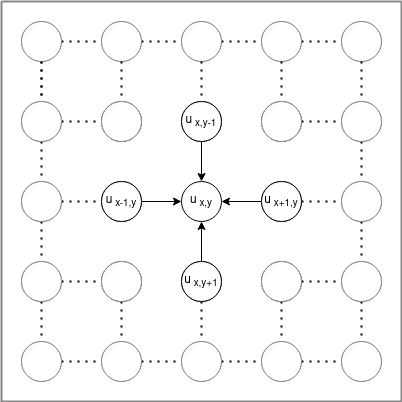
\includegraphics[scale=0.7]{img/5point.png}
    \caption{Temperatūros pasiskirstymas vidiniuose matricos taškuose}
    \label{img:5point}
\end{figure}

Norėdami išspręsti šias lygčių sistemas, naudosime Jakobi iteracinį metodą \cite{burden2011numerical}, kiekvienos iteracijos metu formulės kintamųjų reiškmes keisdami praėjusios iteracijos reikšmėmis.
Laikysime, kad sistema pasiekė galutinę savo būsena, kai taško temperatūrų skirtumas skirtingų iteracijų metu bus mažesnis už norima paklaida.

Kraštinių taškų temperatūros pasiskirstymas nulemia galutinį temperatūros pasiskirstymą erdvėje.
Vidinių taškų pradinis temperatūros pasiskirstymas įtakos galiniam temperatūros pasiskirstymui neturi, tačiau gali turėti įtakos konvergencijos greičiui.
Kraštinių taškų temperatūra šito tyrimo būdu aprašomą kaip:

\[ f(x, 0) = f(x, N-1) = |sin(x/N * 2\pi * 5/2)| = |sin(\frac{5\pi * x}{N})| \], 

kur N yra matricos kraštinės taškų skaičius.
Ši formulė pirmajai ir paskutinei eilutei priskiria 5 $sin$ bangų teigiamas reikšmes.
Likusiems taškams priskiriama 0 temperatūra.
Šio darbo metu taškams priskiriamos temperatūros reikšmės nuo 0 iki 1 imtinai, taip leidžiant modeliuoti į realia objekto temperatūra taikant paprasta proporcija.
Vizualiai pradinis temperatūrų pasiskirstymas matomas \ref{img:start} paveikslėlyje.
Juodi taškai atitinka 1 reikšmę, balti - 0.
Uždavinio tikslas - nustatyti galutinį temperatūros pasiskirstymą plokštelėje, kai temperatūra plokštelėje nebekinta.
Leistina paklaida (temperatūros skirtumas kuri pasiekus laikysime kad programa pasiekė galutinę savo būseną) šio tyrimo eksperimentų metu buvo 0.001.  
Vizualiai galutinis temperatūros pasiskirstymas matomas \ref{img:end} paveikslėlyje.
Laikas per kurį temperatūra pasiskirsto erdvėje, erdvė sudarančios medžiagų šiluminis laidumas šiame darbe nėra nagrinėjami. 

\begin{figure}[H]
    \centering
    
\includegraphics[scale=0.7]{img/image_0000000.png}
    \caption{Pradinis temperatūros pasiskirstymas}
    \label{img:start}
\end{figure}

\begin{figure}[H]
    \centering
    
\includegraphics[scale=0.7]{img/image_1000000.png}
    \caption{Galutinis temperatūros pasiskirstymas plokštelėje}
    \label{img:end}
\end{figure}

\section{Šilumos uždavinio sprendimas}

Šiame skyriuje nagrinėjamas programinis šilumos uždavinio sprendimas.


\subsection{Programos testavimo aplinka}

Siekiant išlaikyti vienodas sąlygas ir ištestuoti algoritmą turint didelį centinių procesorių kiekį, visi šiame darbe aprašyti eksperimentai buvo vykdomi Vilniaus Universiteto Matematikos ir Informatikos fakulteto Skaitmeninių tyrimų ir skaičiavimų centro paskirstytų skaičiavimų tinkle.
Šio darbo rašymo metu buvo naudojamas „beta“ telkinys, kurį sudaro 56 (testavimo metu praktiškai buvo pasiekiami tik 42) mazgai turinys po 2 Intel Xeon X5650 procesorius, kurių kiekvienas turi po 6 branduolius. 
Kiekviename mazge yra 24 GB operatyviosios atminties (ang. RAM) ir jie turi prieigą prie 20Gbit/s infiniband tinklo.
Skaičiavimų tinkle buvo instaliuota Debian operacinė sistemą, lygiagrečiam algoritmui buvo naudojamas OpenMP bibliotekos 6.3.0 versija.
Programoms paleisti buvo naudojama sistemoje esanti „Slurm“ užduočių valdymo sistema ir „short“ užduočių eilė, turinti 2 valandų ir 2 GB vienam naudojamam branduoliui limitą.

\subsection{Nuoseklusis algoritmas}

Nuoseklusis algoritmas įgyvendintas C++ kalba. 
Algoritmo pradžioje alokuojama atmintis dviems N*N dydžio masyvams, kur N yra matricos kraštinės ilgis: viename saugoma dabartinė matricos būsena, kitas yra pildomas naujomis reikšmėmis iteracijos metu.
Naudojami vienmačiai masyvai, nes didžioji dalis OpenMPI bibliotekos funkcijų, kuri buvo naudotos lygiagretinant algoritmą, tikisi vienmačių masyvų duomenų perdavimui, o nuoseklaus algoritmo veikimui vienmačių ir dvimačių masyvų naudojimas nedaro didelės įtakos algoritmo veikimo laikui.
Pirmasis masyvas užpildomas pradine matricos būsena, tada pradedamas iteracinis procesas, kai kiekvienos iteracijos metu, kiekvienam vidiniam matricos taškui yra priskiriama reikšmė, lygi jį supančių 4 taškų vidurkiui, o kraštinės matricos reikšmės nekinta.
Taip pat iteracijos metu fiksuojamas maksimalus temperatūros pasikeitimas, skirtas nustatyti ar matrica pasiekė galutinė savo būseną.
Ši reikšmė kiekvienos iteracijos palyginama su nustatyta paklaidos reikšme ir jei temperatūros pasikeitimas yra mažesnis už leistina paklaida, laikome kad matrica pasiekė pasavo galutinį temperatūrų pasiskirstymą.

Testuojant nuoseklųjį algoritmą su skirtingais matricos kraštinės ilgio reikšmėmis (\ref{table:seq_time} lentelė), pastebėta kad algoritmo vykdymo laikas logoritmiškai priklauso matricos kraštinės ilgio.
Padidinus kraštinės ilgį beveik 2 kartus, vykdymo laikas padidėja beveik 4 kartus, nes algoritmas nagrinėja šilumos pasiskirstymą dvimatinėje erdvėje, todėl padidinus matricos kraštinės ilgį 2 kartus, duomenų kiekis padidėja 4 kartus.
Matricos kraštinės ilgiai pasirinkti dvejeto laipsniai + 2, kad lygiagretinant algoritmą vidinės matricos reikšmes būtų padalinti skirtingiems procesams vienodais kiekiais. 
Pridedamos dvi eilutės šiame skaičiavime atitinka dvi matricos kraštines - eilutes ir stulpelius kurių temperatūrų reikšmės nekinta.
Testuojant nuoseklųjį algoritmą, kai matricos kraštinę sudaro 8194 taškai, buvo pasiektas sistemos užduočių vykdymo laiko limitas (2 valandos).



\begin{table}[]
    \begin{tabular}{|r|rrrr|}
        \hline
        \multicolumn{1}{|l|}{\multirow{2}{*}{Matricos kraštinė}} & \multicolumn{4}{l|}{Vykdymo laikas (s)}                                                                                                     \\ \cline{2-5}
        \multicolumn{1}{|l|}{}                                   & \multicolumn{1}{l|}{Bandymas 1}         & \multicolumn{1}{l|}{Bandymas 2} & \multicolumn{1}{l|}{Bandymas 3} & \multicolumn{1}{l|}{Vidurkis} \\ \hline        258                                                      & \multicolumn{1}{r|}{7.71}               & \multicolumn{1}{r|}{7.712}                     & \multicolumn{1}{r|}{7.815}      & 7.746                         \\ \hline
        250                                                      & \multicolumn{1}{r|}{7.710}              & \multicolumn{1}{r|}{7.712}      & \multicolumn{1}{r|}{7.815}      & 7.746                         \\ \hline
        514                                                      & \multicolumn{1}{r|}{35.243}             & \multicolumn{1}{r|}{34.921}     & \multicolumn{1}{r|}{34.721}     & 34.962                        \\ \hline
        1026                                                     & \multicolumn{1}{r|}{140.821}            & \multicolumn{1}{r|}{141.342}    & \multicolumn{1}{r|}{140.621}    & 140.928                       \\ \hline
        2050                                                     & \multicolumn{1}{r|}{577.458}            & \multicolumn{1}{r|}{572.498}    & \multicolumn{1}{r|}{582.138}    & 577.365                       \\ \hline
        4098                                                     & \multicolumn{1}{r|}{2393.624}           & \multicolumn{1}{r|}{2421.341}   & \multicolumn{1}{r|}{2362.241}   & 2392.402                      \\ \hline
    \end{tabular}
    \caption{Nuoseklaus algoritmo vykdymo laikas}
    \label{table:seq_time}
\end{table}


\subsection{Lygiagretieji algoritmai}

Pradžiai apibrėšime kriterijus, pagal kurios bus vertinamas lygiagretus algoritmas.
Vienas iš pagrindinių vertinimo kriterijų yra algoritmo pagreitėjimas, nusakantis kiek kartų greičiau lygiagretus algoritmas, naudojantis $p$ branduolių, įvykdo užduotį už nuoseklųjį algoritmą \cite{eager1989speedup}.   
Algoritmo pagreitėjimas vertinamas kaip:

\[ S(p) = \frac{t_s}{t_p} ,\]

kur $p$ yra procesorių skaičius, $t_s$ -  geriausias nuoseklaus algoritmo vykdymo laikas, $t_p$ - lygiagretaus algoritmo, naudojančio p procesorių, vykdymo laikas. 

Maksimalus įmanomas teorinis pagreitėjimas gali būti tiesinis. 
Tai galėtų būti pasiekta duomenys yra padalinami į vienodas dalis, o komunikacijos tarp procesų nevyksta.
Tuomet pagreitėjimas yra lygus procesorių skaičiui:

\[ S_{max}(p) = \frac{t_s}{t_s/p} = p .\]

Jei lygiagretaus algoritmo pagreitėjimo reikšmė yra didesnė nei procesorių skaičių - $S(p) > p$ - pasiekiamas supertiesininis (ang. superlinear) pagreitėjimas. 
Tai gali atsitikti dėl neoptimaliai įgyvendinto nuoseklaus algoritmo, arba netiksliai įgyvendinto lygiagretaus algoritmo, kai yra praleidžiami žingsniai.

Maksimalus praktinis algoritmo pagreitėjimas priklauso nuo algoritmo dalies, kuri gali būti išlygiagretinamas. 
Jei algoritmo dalį, kuri negali būti išlygiagretinama, pažymėsime $f$ ($0 \le f \le 1$), trumpiausias lygiagrečios programos vykdymo laikas bus lygus $f*t_s+ (1-f)*t_s/p$, o maksimalus pagreitėjimas apibrėžiamas kaip Amdahl'o dėsnis \cite{amdahl1967validity}:



\[ S(p) = \frac{t_s}{f*t_s+ (1-f)*t_s/p} = \frac{p}{1+(p-1)f} .\]


Šiame darbe nagrinėjamo lygiagretaus algoritmo nuosekliojoje dalyje (t.y. dalyje kuri nėra išlygretinama) vyksta tik konfiguracinių parametrų nuskaitymas. 
Taip pat nėra lygiagretinamas paketų užkrovimas ir kitos prieš pagrindinės (ang. main) programos funkcija iškvietimą vykstančios operacijos, tačiau tai nedaro įtakos algoritmo tyrimui, nes laiko matavimas pradedamas tik iškvietus pagrindinę programos funkciją.
Matricos kraštines suskaidžius į 2050 taškų, nuoseklaus algoritmo konfiguracijos nuskaitymas vidutiniškai truko 0,002 sekundes (žymėsime $t_{np}$), kai tuo metu likusieji skaičiavimai vidutiniškai užtruko 577,363 sekundes.
Toks laiko santykis reikia kad nelygiagretinama algoritmo dalis yra:

\[ f = \frac{t_{np}}{t_p} = \frac{0,002}{0,002+577,363} \approx 0.00000346 .\]

Šis įvertis reiškia, kad maksimalus algoritmo pagreitėjimas naudojant begalinį skaičių procesorių bus lygus:

\[ \underset{p \rightarrow \inf}{S(p)} = \frac{1}{f} = \frac{1}{0.00000346} \approx 289017  ;\]

o tai reiškia neišlygegretinama algoritmo dalis turės įtakos lygiagretaus vykdymo laikui tik naudojant labai didelį procesų kiekį.

\begin{figure}[H]
    \centering
    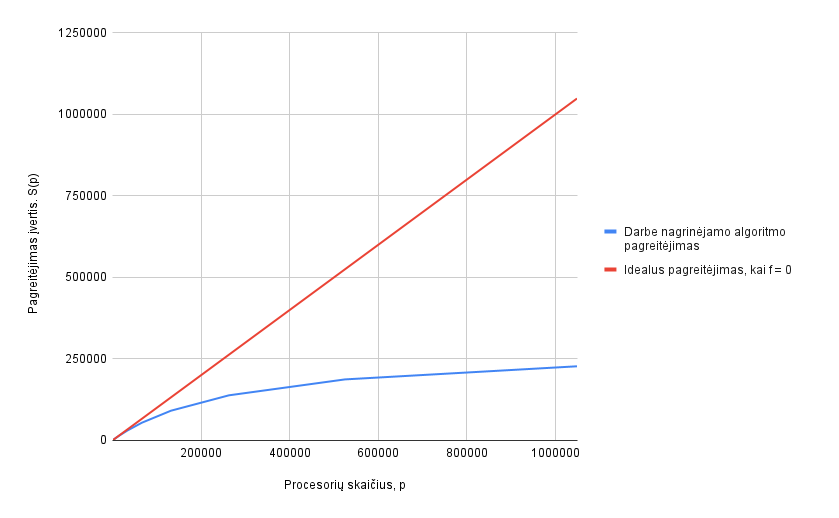
\includegraphics[scale=0.5]{img/max_speedup.png}
    \caption{Maksimalus lygiagretaus algoritmo pagreitėjimo įverčio priklausomybė nuo procesorių skaičiaus}
    \label{img:max_speedup}
\end{figure}

Maksimalaus pagreitėjimo reiškmes naudojant skirtus procesorių kiekius matomos \ref{img:max_speedup} grafike.
Šio darbo ribose algoritmas nebus tiriamas naudojant labai didelį procesorių kiekį, todėl net ir naudojant maksimalų procesorių kiekį (256),
maksimalus pagreitėjimo reikšme bus artima procesorių skaičiui ($S(256) \approx 255.774$), todėl neišlygegretinta algoritmo dalis neribos algoritmo pagreitėjimo.  

Taip pat lygiagretiems algoritmams vertinti naudojama efektyvumo metrika \cite{eager1989speedup}.
Darant prielaidą, kad nuoseklusis algoritmas visada efektyviai išnaudoja jam priskirto procesoriaus resursą, efektyvumo metrika parodo kokia laiko dalį nuoseklusis sprendimas išnaudoja jam priskirtus procesorius.
Efektyvumas, dažniausiai žymimas reide $E$, matematiškai išreiškiamas kaip nuoseklaus algoritmo ir lygiagretaus algoritmo padauginto iš naudotų branduolių skaičiaus vykdymo laiko santykis:

\[ E = \frac{t_s}{t_p * p}\]

Taip pat efektyvumą galime išreikšti per algoritmo pagreitėjimą:

\[ E = \frac{S(p)}{p}\]

Įdealiu atveju, esant maksimaliam algoritmo pagreitėjimui $S(p)=$" algoritmo efektyvumas bus lygus 1. Tai pasiekiama kai visi procesoriai visa laiką yra išnaudojami skaičiavimo užduotims. 


\subsection{Duomenų dalinimas eilutėmis}

Viena iš duomenų paskirstymo lygiagrečiajam algoritmui strategijų yra duomenis paskirstyti eilutėmis (arba stulpeliais).
Norint $N*N$ dydžio matricos duomenis padalint duomenis $p$ procesams, kiekvienam procesui programos vykdymo pradžioje priskiriama po  $(\frac{N-2}{p}+2) * N$ taškų. 
$N-2$ atitinka vidinių matricos stulpelių kiekį, kuris kinta laikui bėgant (2 atitinka išorinius matricos stulpelius turinčius pastovią temperatūrą). 
Ši reikšmė padalinama iš procesų skaičiaus, ir kiekvienas procesui priskiriamos po 2 papildomas eilutes kurios yra naudojamos vidinių reikšmių skaičiavimui (\ref{img:distribution} paveikslėlis).
\begin{figure}[H]
    \centering
    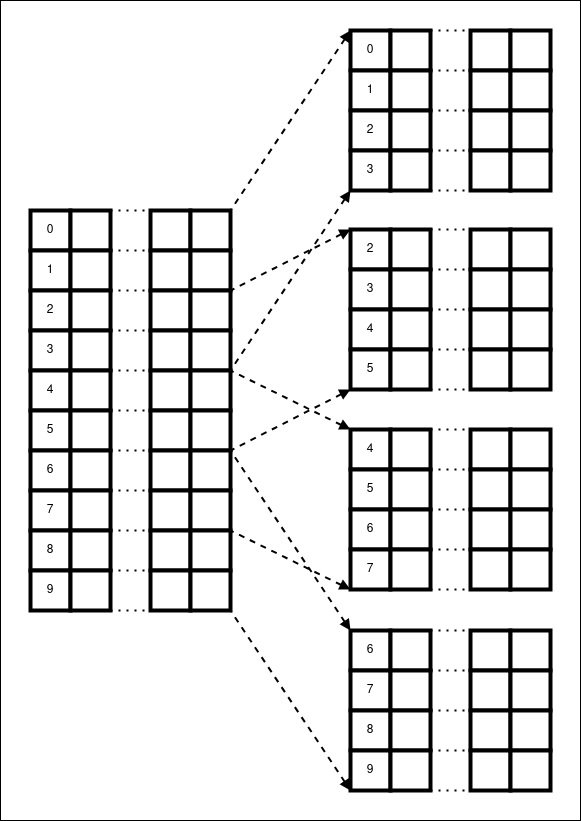
\includegraphics[scale=0.4]{img/distribution.png}
    \caption{Duomenų padalinimas. 10 eilučių padalinamos 4 procesams.}
    \label{img:distribution}
\end{figure}


Naudojant Jakobi iteracinį metodą, kiekvienos iteracijos metu, pirmos ir paskutinės padalintų eilučių reikšmės turi būti sinchronizuojamos tarp gretimas matricos dalis apdorojančių procesų \ref{img:sync}. 
Pirmasis ir paskutinis procesas šonines reikšmės sinchornizuoja tik su vienu iš procesu, nes viena iš jas sudarančių matricos eilučių atitinka pradinės matricos kraštines eilutes, turinčias pastovias reikšmes.

\begin{figure}[H]
    \centering
    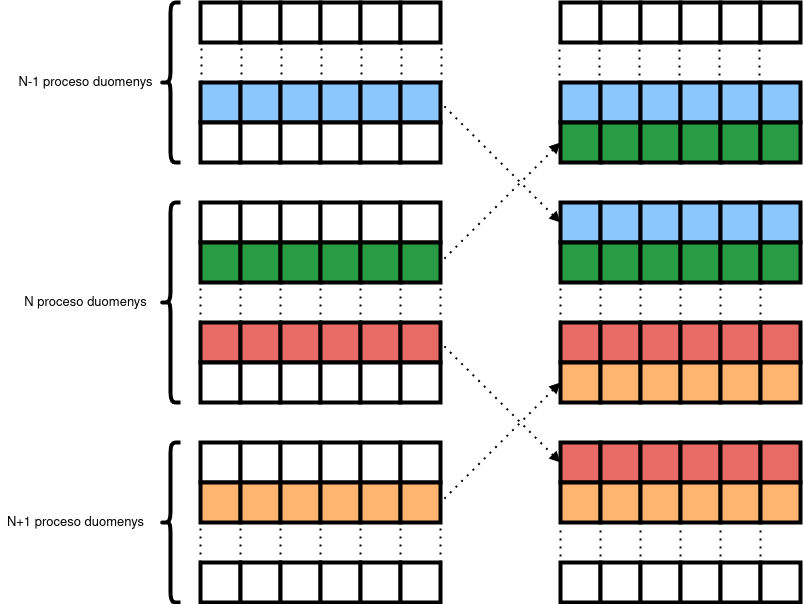
\includegraphics[scale=0.5]{img/sync.png}
    \caption{Duomenų synchronizacija tarp skirtingų procesų}
    \label{img:sync}
\end{figure}

Norint nustatyti, kada didžiausias temperatūrų iteracijų skirtumas pasiekė norimą reikšmę ir reikia nustoti vykdyti programą, kiekvienoje proceso iteracijos pabaigoje suskaičiuoja didžiausią lokalų temperatūros pokytį ir jį siunčia pagrindinam procesoriui, 
kuris gavęs visas reišmes, įvertiną ar bent vienas procesoriaus lokalus skirtumas viršyja norima paklaidą, ir nusprendžia ar tęsti iteravimą.
Norint išvengti visuotinio sinchronizavimo tarp visų branduolių ir pagrininio proceso kiekvienos iteracijos metu, maksimlaus pokyčio reikšmių siuntimas ir palyginimas vykdomas tik kas 100 iteracijų.

\subsection{Lygiagretaus algoritmo, kai duomenys padalinimo eilutėmis, analyzė}


Lygiagretaus algoritmo veikimo laiko įverčiai, kai matricos kraštinę sudoro 2050 taškų pateikiami \ref{table:parallel2050} lentelėje. 
Prieš testuojant lygiagretūjį algoritmą pakeitus branduolių skaičių, buvo atliekamas testinis paleidimas, kurio vykdymo laikas nėra įtrauktas į šią lentelė. 
Testinio paleidimo yra skirtas užtikrinti kad visi užduočiai reikalingi mazgai nebūtų miego busenoje (ang. Hibernation) ir būtų pasiruošę vykdyti algoritmą.

Kaip matoma \ref{img:parallel_time} grafike, vykdymo laikas atvirkšiai priklauso nuo naudojamų branduolių skaičiaus.

\begin{table}[H]
    \begin{tabular}{|r|rrrr|}
        \hline
        \multicolumn{1}{|l|}{\multirow{2}{*}{Branduolių skaičius}} & \multicolumn{4}{l|}{Vykdymo laikas (s)}                                                                                                     \\ \cline{2-5}
        \multicolumn{1}{|l|}{}                                     & \multicolumn{1}{l|}{Bandymas 1}         & \multicolumn{1}{l|}{Bandymas 2} & \multicolumn{1}{l|}{Bandymas 3} & \multicolumn{1}{l|}{Vidurkis} \\ \hline
        2                                                          & \multicolumn{1}{r|}{304.223}            & \multicolumn{1}{r|}{302.624}    & \multicolumn{1}{r|}{302.871}    & 303.239                       \\ \hline
        4                                                          & \multicolumn{1}{r|}{157.587}            & \multicolumn{1}{r|}{157.362}    & \multicolumn{1}{r|}{158.112}    & 157.687                       \\ \hline
        8                                                          & \multicolumn{1}{r|}{87.142}             & \multicolumn{1}{r|}{87.452}     & \multicolumn{1}{r|}{88.655}     & 87.750                        \\ \hline
        16                                                         & \multicolumn{1}{r|}{52.371}             & \multicolumn{1}{r|}{51.578}     & \multicolumn{1}{r|}{52.713}     & 52.221                        \\ \hline
        32                                                         & \multicolumn{1}{r|}{29.452}             & \multicolumn{1}{r|}{28.826}     & \multicolumn{1}{r|}{30.192}     & 29.490                        \\ \hline
        64                                                         & \multicolumn{1}{r|}{16.897}             & \multicolumn{1}{r|}{17.044}     & \multicolumn{1}{r|}{16.454}     & 16.798                        \\ \hline
        128                                                        & \multicolumn{1}{r|}{10.299}             & \multicolumn{1}{r|}{9.956}      & \multicolumn{1}{r|}{9.844}      & 10.033                        \\ \hline
        256                                                        & \multicolumn{1}{r|}{6.027}              & \multicolumn{1}{r|}{6.078}      & \multicolumn{1}{r|}{6.028}      & 6.044                         \\ \hline
    \end{tabular}
    \caption{Lygiagretaus algoritmo vykdymo laikas, kai matricos kraštinę sudaro 2050 taškų}
    \label{table:parallel2050}
\end{table}

\begin{figure}[H]
    \centering
    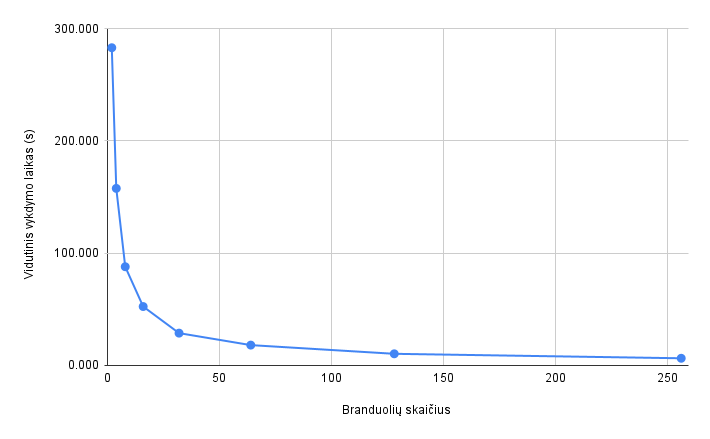
\includegraphics[scale=0.5]{img/parallel_time.png}
    \caption{Lygiagretaus algoritmo vykdymo laikas priklausomybė nuo naudojamų branduolių skaičiaus, kai matricos kraštinę sudaro 2050 taškų}
    \label{img:parallel_time}
\end{figure}


Taip pat lygiagretus algoritmas buvo testuojamas kai matricos kraštinę sudarė 16386 taškai, vykdymo laikas matomas \ref{table:parallel16386} lentelė.
Testuojant naudojant 64 ar mažiau branduolių, programos veikimo laikas viršijo 2 valandas, ir programa buvo sustabdyta. 
Naudojant šią matricos kraštinės reikšmę nuosekliojo algoritmo programa viršydavo sistemos atminties limitą (2GB 1 branduoliui).




\begin{table}[]
    \begin{tabular}{|l|lrrr|}
        \hline
        \multirow{2}{*}{Branduolių skaičius} & \multicolumn{4}{l|}{Vykdymo laikas (s)}                                                                                                     \\ \cline{2-5}
                                             & \multicolumn{1}{l|}{Bandymas 1}         & \multicolumn{1}{l|}{Bandymas 2} & \multicolumn{1}{l|}{Bandymas 3} & \multicolumn{1}{l|}{Vidurkis} \\ \hline
        \multicolumn{1}{|r|}{128}            & \multicolumn{1}{r|}{4419.302}           & \multicolumn{1}{r|}{4403.089}   & \multicolumn{1}{r|}{4418.429}   & 4413.607                      \\ \hline
        \multicolumn{1}{|r|}{256}            & \multicolumn{1}{r|}{2464.156}           & \multicolumn{1}{r|}{2421.661}   & \multicolumn{1}{r|}{2468.414}   & 2451.410                      \\ \hline
        
    \end{tabular}
    \caption{Lygiagretaus algoritmo vykdymo laikas, kai matricos kraštinę sudaro 16386 taškai}
    \label{table:parallel16386}
\end{table}



\begin{table}[]
    \begin{tabular}{|r|r|r|r|}
        \hline
        \multicolumn{1}{|l|}{Branduolių skaičius} & \multicolumn{1}{l|}{Vykdymo laikas} & \multicolumn{1}{l|}{Pagreitėjimas, $S(p)$} & \multicolumn{1}{l|}{Efektyvumas, $E(p)=\frac{S(p)}{p}$} \\ \hline
        1                                         & 577.365                             & 1                                          & 1                                                       \\ \hline
        2                                         & 303.239                             & 1.903991127                                & 0.95                                                    \\ \hline
        4                                         & 157.687                             & 3.661462264                                & 0.92                                                    \\ \hline
        8                                         & 87.750                              & 6.579683114                                & 0.82                                                    \\ \hline
        16                                        & 52.221                              & 11.05625487                                & 0.69                                                    \\ \hline
        32                                        & 29.490                              & 19.57833164                                & 0.61                                                    \\ \hline
        64                                        & 16.798                              & 34.37037405                                & 0.54                                                    \\ \hline
        128                                       & 10.033                              & 57.54659623                                & 0.45                                                    \\ \hline
        256                                       & 6.044                               & 95.52170077                                & 0.37                                                    \\ \hline
    \end{tabular}
    \caption{Lygiagretaus algoritmo pagrėitėjimas ir efektyvumas. }
    \label{table:speedup}
\end{table}

\begin{figure}[H]
    \centering
    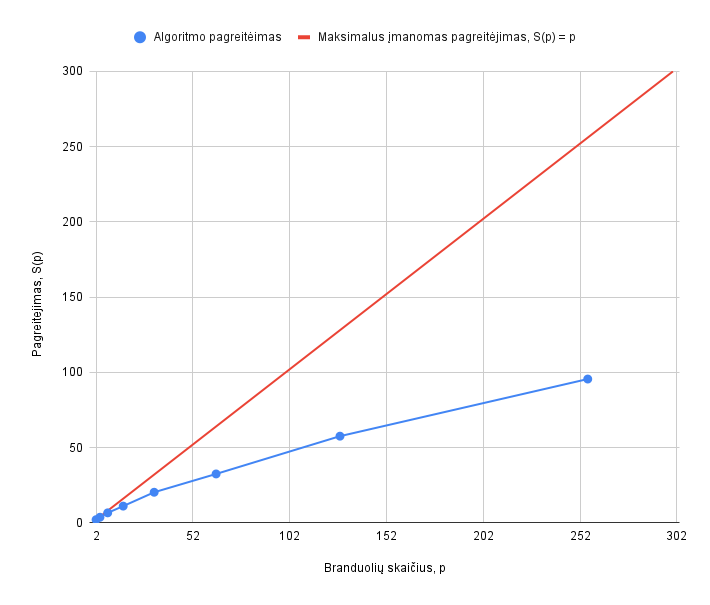
\includegraphics[scale=0.5]{img/parallel_speedup.png}
    \caption{Lygiagretaus algoritmo pagreitėjimo priklausomybė nuo naudojamų branduolių skaičiaus, kai matricos kraštinę sudaro 2050 taškų}
    \label{img:parallel_speedup}
\end{figure}


\ref{img:parallel_speedup} grafike matomas lygiagretaus algoritmo logoritminis pagreitėjimas, tačiau Amdahl'o dėsnio \cite{amdahl1967validity} apibrėžiamas maksimalus pagreitėjimas nėra pasiekiamas - naudojant tokį branduolių kiekį pagreitėjimas turėtų būti artimas idealiam pagreitėjimui  $S_{max}(p)=p$.
Tai galimai nutinka dėl to, kad Amdahl'o dėsnis neatisižvelgia į komunikacijos tarp skirtingų procesorių kaštus.
Tikslų programos skaičiavimų ir komunikacijos santykį įvertinti yra sunku, nes komunikacijos laikas gali skirtis laikas prikausomai ar komunikuojantys procesai naudoja to pačio ar skirtingų centrinių procesorių branduolius, 
ir ar centriniai procesoriai yra toje pačioje ar skirtinguose motininėse plokštelėse. 
Tas iš dalies matoma \ref{table:speedup} lentelėje, kad algoritmo efektyvumas naudojant 2 ir 4 branduolius yra artimas 1, o naudojant daugiau branduolių lygiagretaus sprendimo efektyvumas mažėja.
Tai galima sieti su tuo kad testavimui naudoto paskirstytų skaičiavimų tinklo mazguose naudojami procesoriai, turinys 6 branduolius, todėl naudojant 2 ir 4 branduolius didelė tikimybė, kad bus naudojamas 1 fizinis procesorius, taip išvengiant didelių komunikacijos kaštai tarp atsikirų procesų.
Taip pat, \ref{table:speedup} lentelėje matomas algoritmo efektyvumo mažėjimas didinant branduolių skaičių, iš to galime daryti prielaidą, kad pradinius duomenis skaidant į vis mažesnes dalis, vis didesnę algoritmo vykdymo laiką užima komunikacija tarp skirtingus duomenis apdorojančių procesų.
Nors testuojant su vis didesnių branduolių skaičiumi algoritmo efektyvumas mažėja, lygiagretaus algoritmo pagreitėjimo metrika didinant naudojamų branduolių nenustoja didėti, iš to galima daryti prielaidą šių testų metu nebuvo rastas branduolių skaičius, kurį naudojant komunikacijos kaštai nusvertų gautą algoritmo pagreitėjimą, kai užduotis yra padalinama į mažesnes dalis. 

% Medžiagos darbo tema dėstymo skyriuose pateikiamos nagrinėjamos temos detalės: pradinė me-
% džiaga, jos analizės ir apdorojimo metodai, sprendimų įgyvendinimas, gautų rezultatų apibendrinimas.
% Šios dalies turinys labai priklauso nuo darbo temos. Kursiniame darbe analizuojama dalykinė sritis, jo
% rezultate formuluojamas bakalauro darbe sprendžiamas uždavinys. Referatas neatitinka kursiniams
% darbams keliamų reikalavimų. Dėstymo skyriai gali turėti poskyrius ir smulkesnes sudėtines dalis, kaip
% punktus ir papunkčius

% Medžiaga turi būti dėstoma aiškiai, pateikiant argumentus. Tekste dėstomas
% trečiuoju asmeniu, t.y. rašoma ne „aš manau“, bet „autorius mano“, „autoriaus
% nuomone“. Reikėtų vengti informacijos nesuteikiančių frazių, pvz., „...kaip jau
% buvo minėta...“, „...kaip visiems žinoma...“ ir pan., vengti grožinės
% literatūros ar publicistinio stiliaus, gausių metaforų ar panašių meninės
% išraiškos priemonių.


\sectionnonum{Rezultatai ir išvados}

Šio darbo rašymo metu buvo implementuoti nuoseklusis ir lygiagretusis algoritmai, spendžiantys šilumos pasiskirstymo užduotį Jacobi iteraciniu metodu naudojant baigtinių skirtumų schemą.
Abu algoritmai buvo ištestuoti naudojant prieinamus MIF superkompiuterio resursus, lygiagretusis algoritmas buvo testuojamas naudojant iki 256 branduolių.
Naudojant lygiagretųjį algoritmą, buvo išspręstas uždavinys, kurio dėl sistemų resursų apribojimų nebuvo įmanoma išspręsti nuosekliuoju algoritmu. 
Buvo pasiektas lygiagrečiojo algoritmo pagreitėjimas iki 95 kartų, o atlikta pagreitėjimo ir efektyvumo analizė parodė kad naudojant didesnį branduolių kiekį būtų galima dar labiau sutrumpinti skaičiavimo laiką.
Sukurta programa, įgyvendinanti algoritmo sprendimą, yra konfiguruojama, leidžianti lengvai keisti pradines sąlygas ir ją perpanaudoti praktinių uždavinių sprendimams.

Ateityje, norint gauti geresnį lygiagretaus algoritmo pagreitėjimo ir efektyvumo rezultatus, būtų verta pabandyti kitokius duomenų dalinimo būdus, (pvz kvadratais), pabandyti lygiagretizuoti sprendimą naudojant grafinius procesorius.
% \subsection{Poskyris}
% Citavimo pavyzdžiai: cituojamas vienas šaltinis \cite{PvzStraipsnLt}; cituojami
% keli šaltiniai \cite{PvzStraipsnEn, PvzKonfLt, PvzKonfEn, PvzKnygLt, PvzKnygEn,
% PvzElPubLt, PvzElPubEn, PvzMagistrLt, PvzPhdEn}.

% \subsubsection{Skirsnis}
% \subsubsubsection{Straipsnis}
% \subsubsection{Skirsnis}
% \section{Skyrius}
% \subsection{Poskyris}
% \subsection{Poskyris}



% kuriame pateikiami tyrimo objektas ir aktualumas, darbo tikslas, keliami už-
% daviniai ir laukiami rezultatai, tyrimo metodai, numatomas darbo atlikimo procesas, apibūdi-
% nami darbui aktualūs literatūros šaltiniai.
% Pastaba. Darbo uždavinyje apibrėžiamas siekiamas rezultatas, kad būtų galimybė išmatuoti,
% ar tikslai ir uždaviniai yra išspręsti, bei kokiu lygiu (vertinant kiekybę bei kokybę). Pavyz-
% džiui, „Atlikti literatūros .... analizę“ nėra tinkamas uždavinys, nes nusako procesą, tačiau
% neapibrėžia jo rezultato. Tinkamos uždavinio formuluotės šablonai: „Išanalizuoti literatūrą
% ... siekiant apžvelgti ir įvertinti /... metodų tinkamumą sprendžiamam uždaviniui/privalu-
% mus ir trūkumus sprendžiant ... uždavinį/rekomenduojamas ... projektavimo gaires, šablonus
% ir pan.

% \sectionnonum{Įvadas}
% Įvade nurodomas darbo tikslas ir uždaviniai, kuriais bus įgyvendinamas tikslas,
% aprašomas temos aktualumas, apibrėžiamas tiriamasis objektas akcentuojant
% neapibrėžtumą, kuris bus išspręstas darbe, aptariamos teorinės darbo prielaidos
% bei metodika, apibūdinami su tema susiję literatūros ar kitokie šaltiniai,
% temos analizės tvarka, darbo atlikimo aplinkybės, pateikiama žinių apie
% naudojamus instrumentus (programas ir kt., jei darbe yra eksperimentinė dalis).
% Darbo įvadas neturi būti dėstymo santrauka. Įvado apimtis 2 -- 4 puslapiai.

% \section{Medžiagos darbo tema dėstymo skyriai}
% Medžiagos darbo tema dėstymo skyriuose išsamiai pateikiamos nagrinėjamos temos
% detalės: pradiniai duomenys, jų analizės ir apdorojimo metodai, sprendimų
% įgyvendinimas, gautų rezultatų apibendrinimas.


% Skyriai gali turėti poskyrius ir smulkesnes sudėtines dalis, kaip punktus ir
% papunkčius.




% \sectionnonum{Rezultatai ir išvados}
% Rezultatų ir išvadų dalyje turi būti aiškiai išdėstomi pagrindiniai darbo rezultatai (kažkas išana-
% lizuota, kažkas sukurta, kažkas įdiegta) ir pateikiamos išvados (daromi nagrinėtų problemų sprendimo
% metodų palyginimai, teikiamos rekomendacijos, akcentuojamos naujovės).

\printbibliography[heading=bibintoc]  % Šaltinių sąraše nurodoma panaudota
% literatūra, kitokie šaltiniai. Abėcėlės tvarka išdėstomi darbe panaudotų
% (cituotų, perfrazuotų ar bent paminėtų) mokslo leidinių, kitokių publikacijų
% bibliografiniai aprašai. Šaltinių sąrašas spausdinamas iš naujo puslapio.
% Aprašai pateikiami netransliteruoti. Šaltinių sąraše negali būti tokių
% šaltinių, kurie nebuvo paminėti tekste. Šaltinių sąraše rekomenduojame
% necituoti savo kursinio darbo, nes tai nėra oficialus literatūros šaltinis.
% Jei tokių nuorodų reikia, pateikti jas tekste.

% \sectionnonum{Sąvokų apibrėžimai}
% \sectionnonum{Santrumpos}
% Sąvokų apibrėžimai ir santrumpų sąrašas sudaromas tada, kai darbo tekste
% vartojami specialūs paaiškinimo reikalaujantys terminai ir rečiau sutinkamos
% santrumpos.

\end{document}
